\documentclass{article}
\usepackage[margin=3cm]{geometry}
\usepackage{xcolor}
\usepackage{graphicx} % Required for inserting images

\title{Project 2 - CSC111}
\author{Nabiha Tariq, Yusyra Hossain, Eleanor Neal, Ruoshui Deng}
\date{March 2026}

\begin{document}

\maketitle

\section{Introduction}
 
\subsection*{Project Name:}
Bird Species and their Interactions in Toronto in 2025

\subsection*{Project Goal:} 
\textbf{To find which bird species (at Toronto in 2025) interact most frequently across different seasons, where the likelihood of interactions is based on the proximity of observations for each species}

\subsection*{Problem Description}
Platforms like iNaturalist allow users to post animal sightings in local areas and discuss their findings in a global community. Every user-contributed observation, ranging from rare to common species, supports biodiversity science and allows researchers to make discoveries and find patterns. iNaturalist catalogues these observations and shares them with data repositories, enabling analysts to find and use user data.\\ \\
This project draws inspiration from the fact that graphs are used to model things in real life, and after some research, the paper "This town ain't big enough ..." by Gonzalo A. et. al (see References). In this project, we model an ecological system of species. We use real-world bird observation data from iNaturalist to analyze how close species are sighted from one another, and how likely they are to interact. Since the dataset includes precise geographic coordinates for each observation, it allows us to model proximity-based interactions between species and examine how these relationships vary across seasons. \\ \\
This project only focuses on the relationship between bird species in Toronto during the year 2025. This decision was made to ensure computational feasibility and to produce a more focused and interpretable model. \\ \\
The goal for this project is to better understand patterns of species co-occurrence and interaction within an ecosystem. Studying these relationships can provide insight into how ecosystems respond to environmental changes, such as shifts in climate or population dynamics. And, analyzing spatial co-occurrence is a well-established ecological method for modeling potential interactions between species in shared environments (Ramírez-Cruz et al., 2019). So by modelling these interactions between species, we hope to contribute to a deeper understanding of biodiversity interactions in ecosystems. \\ 



\section{Computational Overview} 

\subsection{Datasets}
Our project uses real-world biodiversity observation data obtained from iNaturalist (https://www.inaturalist.org/). It's a platform where users upload sightings of any animal (excluding humans) they spot, along with other information such as observation dates, species names, geographic coordinates (latitude and longitude), and associated metadata.\\ \\
While we originally planned on modelling the relationship for all animals across multiple years and locations, the processing time for such a large dataset took very long, so we restricted the dataset to birds in Toronto in the year 2025. Even after doing that, there were too many observations to make an interpretable model. Thus, we capped our observations at 6000 (randomly selected from the subset of bird observations). \\ \\
Before our analysis, we cleaned the dataset to extract only the variables needed. This includes:
\begin{itemize}
    \item \texttt{species\_guess}: the name of the observed species
    \item \texttt{observed\_on}: the date of the observation
    \item \texttt{latitude} and \texttt{longitude}: the geographic location of the observation
    \item \texttt{image\_url}: a reference image associated with the observation
    \item \texttt{positional\_accuracy}: An integer detailing how precise the spotting was. A larger number indicates the position of the species is less precise.
\end{itemize}
We extracted these by processing the dataset with the pandas library, removing irrelevant columns and filtering out observations. The cleaned dataset is then used to construct a list of Observations, instances of our \texttt{Observation} data class, which we use as the primary data structure for performing computations and generating our graph in the program. The \textt{Observation} class stores a species and organizes its recorded locations by season, allowing us to keep all important information in an easy-to-access way.\\ \\
\textit{\textbf{Note}}: Columns dropped are: "id", "uuid", "observed\_on\_string", "time\_observed\_at", "time\_zone", "user\_id", "user\_login", "user\_name", "created\_at", "updated\_at", "quality\_grade", "url", "image\_url", "sound\_url", "tag\_list", "description", "num\_identification\_agreements", "num\_identification\_disagreements", "captive\_cultivated", "oauth\_application\_id", "private\_place\_guess", "private\_latitude", "private\_longitude", "public\_positional\_accuracy", "geoprivacy", "taxon\_geoprivacy", "coordinates\_obscured", "positioning\_method", "positioning\_device", "scientific\_name", "iconic\_taxon\_name", "taxon\_id", "species\_name"
\\ 


\subsection{Description of Program}

\subsubsection{Overview}
Our program models species interactions using a weighted, undirected graph. 
To model interactions between species, we use a custom 'Graph' class, where each vertex represents a bird species and edges represent the likelihood of interaction between two species. \\ \\ Each 'Vertex' stores: The species name, a reference image (used in visualization), and mapping of neighbouring species to both: Raw co-occurrence counts and interaction likelihood. \\
This graph structure is central to our project, as it allows us to easily model complex, non-hierarchical relationships between species without duplication, unlike a tree structure. \\ \\
The overall architecture of the program can be divided into four main stages: \\
\textbf{(1) Data preprocessing:} The raw CSV dataset is cleaned and filtered using \texttt{pandas} to remove irrelevant attributes and group species together. \\
\textbf{(2) Data transformation:} The cleaned data is converted into a collection of \texttt{Observation} objects, where each object holds all observations of a single species. Each observation organizes its data by season, mapping seasonal categories to lists of timestamped geographic coordinates. \\
\textbf{(3) Graph construction:} Using these \texttt{Observation} objects, the program constructs four separate graphs (one per season). For each season, species are added as vertices, and edges are created by comparing all pairs of species and determining whether they co-occur within a specified geographic threshold using the Haversine Distance Formula and the Jaccard Index (justified by Tatsumi et al., 2025). Each edge stores both the raw number of co-occurrences and a computed interaction likelihood. \\
\textbf{(4) Visualization and interaction:} Instead of displaying the full graph (which would be too large and cluttered), our program extracts a portion of the graph centered on the species selected by the user. This subgraph is filtered based on interaction probability and size constraints to ensure readability. The resulting graph is then visualized using \texttt{networkx} and \texttt{matplotlib}, with additional interactivity like hover-based annotations provided through \texttt{tkinter}, \texttt{mplcursors}, \texttt{io} and \texttt{Pillow}.


\subsubsection{Major Computations}  
We first transform the \textit{cleaned} dataset into a collection of \texttt{Observation} objects. Each observation stores a species name and a mapping from seasons to lists of geographic locations (with associated timestamps) where the species was observed. Seasons are determined by extracting the month from each observation date and categorizing it into Winter, Spring, Summer, or Fall. See \texttt{clean\_data} and \texttt{data\_handle} in \texttt{data\_manipulation.py} for concrete details. \\ \\
Using this processed data, we construct four separate graphs, one for each season. This allows us to analyze how species interactions vary throughout the year.\\ \\
To build each seasonal graph (see \texttt{build\_from\_observations} in \texttt{entities.py}), we first make a 'Vertex' for each species (without duplication using \texttt{pandas} library). Then, we compare all pairs of species observed during that season. For each pair, we compute the geographic distance between all combinations of their recorded observation locations using the Haversine distance formula, which accounts for the Earth's curvature. If two observations, \textit{within a timeline of one season}, fall within a proximity \textbf{threshold of 1.0 kilometre}, we treat this as a potential interaction and record it in the graph by adding an edge between the corresponding species. \textit{It is important to note that we expanded the observation timeline to allow observations seen within the same season to be considered for the likelihood of interaction. Otherwise, the data was too sparse. } \\ \\
Since two species may interact more than once (i.e. there may be more than one edge between species), edges in the graph are weighted: each time two species meet the proximity threshold, the weight of the edge between them is incremented (shown visually too, see below). Thus the weight represents the frequency of co-occurrence, and is the proxy for the likelihood of interaction between species. \\ \\
The resulting graph is undirected, as interactions between species are bidirectional. \\ \\
So the main computations \textbf{in the backend} performed by our program include:
\begin{itemize}
    \item Cleaning and filtering the raw CSV dataset by removing irrelevant columns using pandas.
    \item Grouping rows of the same species using pandas filtering
    \item Transforming new, filtered raw CSV data into structured 'Observation' objects so they can be computed on more efficiently
    \item Creating vertices for the graph by grouping observations based on species and adding in neighbours accordingly
    \item Computing pairwise geographic distances between Observations using the haversine formula to get proximity
    \item Constructing weighted edges between pairs of species, and adding in Vertex neighbours, based on this proximity. Note that here, weights represent the frequency of co-occurrence
    \item Building separate graph structures for each season 
    \item Converting the custom graph structure into a format suitable for visualization using networkx and matplotlib
\end{itemize} 
After constructing the graphs, we allow the user to interact with the data through a graphical interface built using \texttt{tkinter}. The user selects a species \textit{from a drop-down menu} and a season by typing in through the pop-up input windows. Based on this input, the program extracts a subgraph from the seasonal graphs, centred on the selected species, including all neighbouring species it interacts with during that season (see below for more information), making the visualization more interpretable and computationally manageable. \\ \\
For visualization, we use the \texttt{networkx} and \texttt{matplotlib} libraries to generate a network graph, with several enhancements to improve clarity, interactivity, and visual appeal. Rather than displaying simple nodes and edges, we use image-based nodes, probability-based filtering, and extra interactive elements like 'hovering for information', 'dropdown menus', and 'thickened edges to show greater probability', to create a more informative and engaging user experience. \\ \\
Specifically, our frontend performs the following:
\begin{itemize}
    \item Collecting user input (species, season, and proximity threshold) through a custom \texttt{tkinter} interface with \textit{input fields, validation, and a \textbf{searchable} dropdown for species selection with \textbf{real-time} filtering}
    \item Selecting the appropriate seasonal graph based on user input, AND error handling if there is no observation of that species in that season.
    \item Extracting a subgraph centered on the chosen species by limiting total nodes to 50, and the maximum number of each species' neighbour to 4 (i.e. by selecting top interactions)
    \item Scaling edge thickness using a logarithmic function to better represent differences in interaction strength
    \item Displaying nodes as circular images of species using \texttt{Pillow} and \texttt{numpy}
    \item Dynamically loading images from URLs using \texttt{urllib}, with fallback handling for missing or invalid images
    \item Positioning nodes using \texttt{networkx.spring\_layout} to produce a visually balanced graph structure
    \item Adding interactive hover functionality using \texttt{mplcursors}, allowing users to view \textit{all} neighbouring species and interaction probabilities for that specific species
    \item Removing axes and visual clutter to produce a cleaner and more user-friendly visualization
\end{itemize}
These design choices significantly enhance the usability of the program by allowing users to explore complex interaction patterns in a simple way, so it is easier to draw connections between species, fulfilling our goal of the project. 

\subsubsection{How the program shows results in a visual way}
The results of our computation are presented through an interactive graph-based visualization that allows users to explore species (i.e., vertices) relationships directly. In addition, the program includes interactive elements that allow users to explore results with more concrete numbers. Users can select different species and seasons, and extract different subgraphs of the dataset centred on the species. \\ \\
To help with analysis, rather than outputting just numerical results, our program translates the interaction probabilities computed by our program into visual features of the graph. Each vertex represents a species, edge represents likelihood, and edge thickness relies on interaction likelihood (i.e, thicker edges represent stronger interaction probabilities), allowing users to analyze complex relationships easily. \\ \\
Furthermore, users can get detailed interaction data (including neighbouring species and concrete probabilities) by hovering over nodes, allowing users to access deeper insights without cluttering the main visualization. \\ \\
This combination of visual abstraction and interactivity makes the results of our program both accessible and analytically meaningful. \\

\subsubsection{Libraries Used}
Our program relies on several external libraries:
\begin{itemize}
    \item \texttt{pandas}: for efficient CSV processing, filtering, and grouping \\ - see \texttt{data\_handle} and \texttt{clean\_data} in \texttt{data\_manipulation.py} \\
  - we use pandas to read the CSV file into a DataFrame, filter out irrelevant columns, handle missing values, and group observations by species to prepare the data for graph construction
  
    \item \texttt{networkx}: for graph construction and layout algorithms \\ - see \texttt{create\_species\_graph} and \texttt{\_initialize\_graph\_vals} in \texttt{run.py} \\
    - we construct a NetworkX graph from our custom graph structure, and use \texttt{spring\_layout} to compute node positions using a force-directed algorithm, and \texttt{draw\_networkx\_edges} to make edges with varying thickness based on interaction strength
    
    \item \texttt{tkinter}: to vreate user interface
  \\ - see \texttt{create\_species\_graph} and \texttt{display\_window} in \texttt{run.py}
  \\ - we use tkinter to build an interactive user interface, including input fields (\texttt{ttk.Entry}), buttons, and a custom searchable dropdown (using \texttt{Listbox} 

    \item \texttt{matplotlib}: for visualization of the graph
    \\ - see \texttt{\_draw\_images}, \texttt{\_fetch\_image}, and \texttt{\_initialize\_graph\_vals}
    \\ - we use \texttt{pyplot} to create the graph, and \texttt{AnnotationBbox} and \texttt{OffsetImage} to render species images at node positions to display image-based nodes
  
    \item \texttt{numpy} and \texttt{Pillow}: for image processing and rendering \\ - see functions \texttt{make\_circular} in \texttt{utils.py} \\
  - we use numpy arrays and Pillow image processing to apply a circular mask to species images

    \item \texttt{mplcursors} - for interactive hover annotations \\
    - see \texttt{\_setup\_hover} in \texttt{run.py}
    - we import \texttt{cursor} from this library to create the hover-over effect

    \item \texttt{urllibs} - for fetching images from URL \\
    - see \texttt{\_fetch\_images} in \texttt{run.py}
    - we use Request and Error to get images from the dataset to use in the nodes, and successfully handle missing image or not found errors as well
\end{itemize}
These libraries allow for both more efficient computation and a more interactive visualization experience. \\

\subsection{How to run the program}
\subsubsection{Installation Requirements}
Our project is written entirely in Python. To run this program, \texttt{Python Version 3.13.5} is required. In addition, the following external libraries must be installed:
\begin{itemize}
    \item pandas
    \item networkx
    \item matplotlib
    \item numpy
    \item mplcursors
    \item Pillow
    \item io
    \item os
\end{itemize} 
The program also uses the built-in \texttt{tkinter} and \texttt{math} library for graphical user input. Since they are included with standard Python installations, no separate installation is required.


\subsubsection{Datasets}
The dataset used in this project is a CSV file (from iNaturalist) with 6000 observations. The dataset - named \texttt{data.csv} - is included as part of our submission in a compressed (zip) folder, so no external downloads are required. Thus, to run the program, it is just necessary to extract the folder from the zip file, and \textbf{have the dataset in the same folder as the other files}. \\ \\
\textit{\textbf{Note}}: Our program only uses a subset of the dataset. However, no work is required from the user's end, because our code already cleans the dataset and produces a new processed file (\texttt{new\_file.csv}) that is used throughout. Again, all work is automatically handled by the program, so no work is required from the user. Just adding this note in case, because while the program is running, the user might see the new file appear in the folder. 

\subsubsection{Main.py}
To run the program, the user must:
\begin{enumerate}
\item \textbf{Download all libraries} in requirements.txt
\item \textbf{Unzip} the folder \texttt{data}, \textbf{extract the data file} (\texttt{data.csv}) and \textbf{put it in the same directory} as the rest of the files.
\item \textbf{Run the file \texttt{main.py}} (this imports all necessary modules, so no other steps required)
\end{enumerate}
After a few seconds, the user will be prompted with a window to select their species name and a season. Clicking 'Species' will open a new window. Both season and species are chosen through \textbf{drop down menu style}; species also comes with a \textbf{'search' function} so the user can find their desired species faster: 
\begin{figure}[h!]
    \centering
    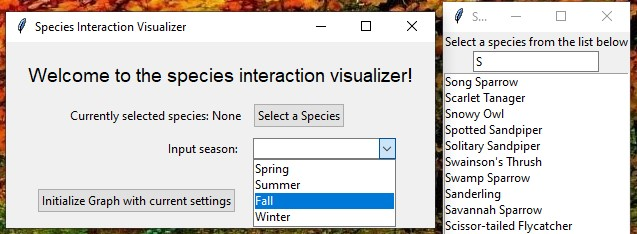
\includegraphics[width=0.75\textwidth]{walkthrough1.jpg}
    \caption{Initial Pop-Up Window}
    \label{fig:myimage}
\end{figure}
\bigskip
\par Once the user selects their desired species and season, they should press the 'Initialize Graph with current settings' button and wait a few seconds. Eventually, a subgraph, centred around the species (see 2.2.2 for implementation details), will show. Interactive features included on the graph include: 
\begin{itemize}
  \item \textbf{Hover Information}: Moving the mouse over any species' node displays a tooltip with detailed likelihood of interactions with neighbouring species, providing exact percentages.
  \item \textbf{Dynamic Interaction}: Nodes are positioned in a layout that ensures minimal overlap and maximizes clarity. The user can explore different nodes to investigate how different species interact across the chosen season.
  \item \textbf{Edge Thickness}: The thickness of edges corresponds to the frequency of co-occurrence, visually highlighting stronger interactions.
  \item \textbf{Zoom In/Out and Pan around}: Users can zoom into any part of the graph, then move it around to analyze the relation between vertices (i.e. co-occurrence) or the thickness of the edges (i.e. likelihood)
  \item \textbf{Save the image}: Users can save any part of the graph as they wish (e.g., zoom into one species and save, or save the whole graph), making it easier to analyze it. \\
\end{itemize}
Thus, this setup provides the user with an interactive and easily interpretable exploration of species co-occurrence.
\begin{figure}[h!]
    \centering
    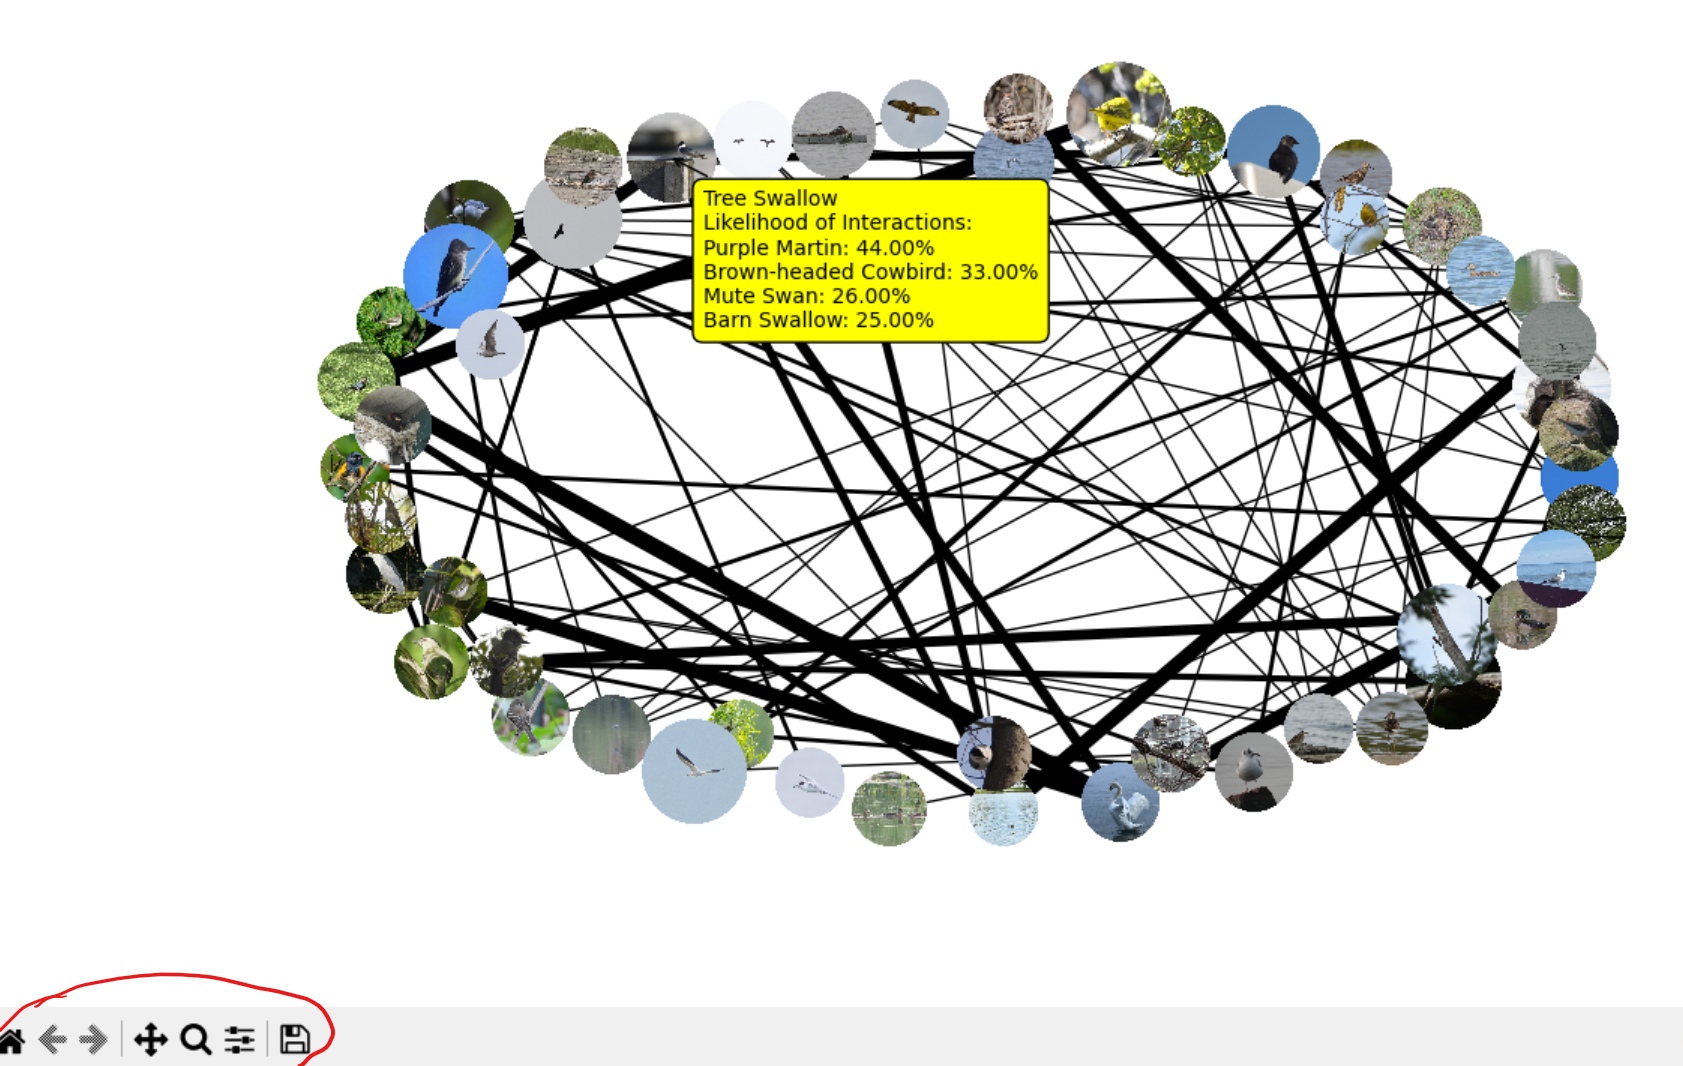
\includegraphics[width=0.75\textwidth]{walkthrough2.png}
    \caption{Full Graph}
    \label{fig:myimage}
\end{figure}
\begin{figure}[h!]
    \centering
    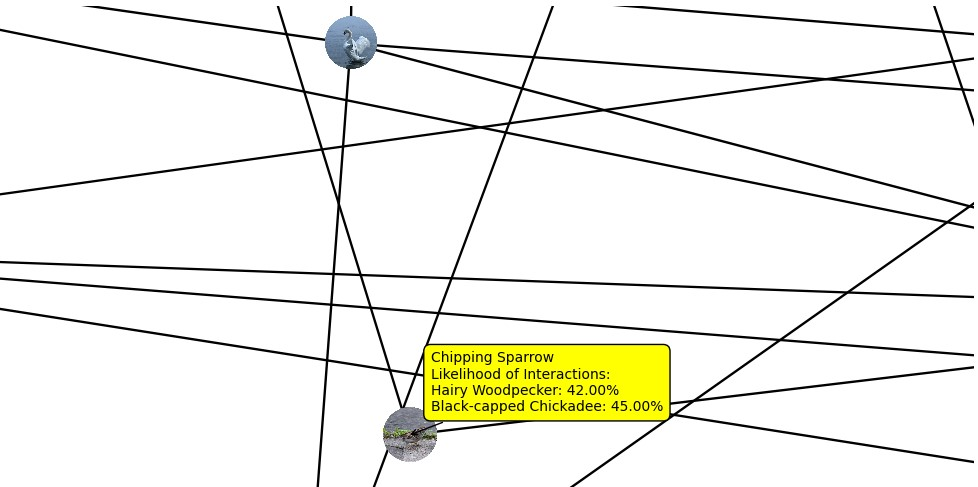
\includegraphics[width=0.75\textwidth]{walkthrough3.jpg}
    \caption{Zoomed In}
    \label{fig:myimage}
\end{figure}

\clearpage

\section{Changes to Computational Plan}
While our overall project remained consistent with the original proposal, we refined several parts of the computational plan to address implementation challenges and Phase 1 feedback we received.\\ \\ 
One major piece of feedback was to consider narrowing down the dataset, since our original dataset contained an extremely large number of observations (about 299,705,908). Visualizing all of these at once would also make the graph cluttered and difficult to interpret. In response, we restricted the dataset to birds only and, instead of displaying the entire graph, we limited the visualization to a user-selected species and its immediate interactions (i.e. neighbours). This approach made the visualization more manageable, and it allows for meaningful insights to be extracted from the data as well (since the user can see the connections better). \\ \\
Another important suggestion from the TA was to clearly define the thresholds used to determine interactions between species. In our proposal, we didn't have a specific number or timeline. So in our final implementation, we addressed this by introducing a geographic threshold of 1 km by computing distances using the haversine formula in one season (3 months). Thus, we added a consistent method for identifying when two species are likely to interact.\\ \\ 
In addition, we expanded on the interactivity and UI of the program. Based on feedback suggesting user driven exploration, we implemented a hover functionality that allows users to view detailed interaction probabilities between species, as well as a searchable species selection interface to efficiently navigate the large dataset. These features improve the usability of the visualization.
We also added images to each node as suggested, enhancing the visual representation of species in the graph. Additionally, we had to implement a probability-based filtering when showing the graph to the user (i.e., limit the number of nodes by only keeping interactions with more than 2\% probability) to keep it readable. \\ \\ 
We also refined our interaction modelling. In the initial proposal, we weren't clear on how we would determine the probability of co-occurrence; we eventually switched from raw co-occurrence counts to a probabilistic prediction using the Jaccard Index (see Tatsumi et al., 2025). \\ \\
Another important change we had to implement was how we classified a possible interaction in the first place. While the original plan was to only count co-occurrence if the species were seen in the same \textit{day} within 1 km, this either required too large of a dataset or produced a graph with few to no vertices. So in the final version of our project, we count co-occurrence if the species were seen in the same \textit{season} within 1 km. \\ \\
Finally, while the original proposal suggested using Plotly for visualization, we instead used NetworkX and Matplotlib. This change was made to better integrate with our custom graph structure and allow more direct control over graph construction and rendering.\\ \\
Overall, these changes improved the visual clarity and computational feasibility of our project. \\ \\



\section{Discussion}
\subsection*{Meeting Project Goal}
The goal of our project is to determine which bird species in Toronto in 2025 are most likely to interact with each other across different seasons, where interaction likelihood is defined based on proximity (1 km) and temporal overlap of observations. \\ \\
By modelling species as vertices and interactions as weighted edges, our graph-based approach successfully captures patterns of co-occurrence. Features such as hover-based interactions and the thickness of edges details enable users to quickly identify the strongest relationships. And in particular, the use of the Jaccard Index allows us to accurately predict interactions (i.e. making it possible to identify which species are more strongly associated with one another, even when the number of total observations differs significantly between species). \\\\ 
The interactive visualization lets users select a species and season, and then explore a centered subgraph, thus \textbf{making it possible to investigate local interaction structures within the larger ecosystem}. By comparing across seasons, users can also identify things like potential ecological overlap, going beyond our goal. \\


\subsection*{Obstacles and Limitations}
Throughout this project, we encountered several technical and design challenges. Some include: 
\begin{itemize}
\item Figuring out how to represent all the nodes and all the relationships between animals. Initially, we had an extremely dense graph (too much edge crossings), making it difficult to extract any meaningful insights. So we added a maximum node limit (50 nodes), a minimum interaction probability threshold (2\%), and limited each node to its top 4 interacting neighbours. To prevent a sparse graph (since the graph is now cut), we also had to expand the co-occurrence window from allowing observations within the same day to the same season. Creating these restrictions were necessary to makle the graph interpretable.
\item Stabilizing our probability of interaction formula. Initially, we relied on raw co-occurrence counts, but it was inconsistent due to different observation frequencies. So, we transitioned to using the Jaccard Index, but this introduced several issues, including zero probabilities and extremely small values. So we added test cases for it and had to refine the formula to ensure correctness.
\item Runtime of the fuction was too long. We addessed that by cutting observations and removing dead code.
\item Data quality and inconsistency. Since the dataset is user-generated, it contains missing values and non-standard characters. Thus we implemented strong error handling to prevent crashes, including fallback mechanisms for missing images and species with no neighbours, checks for incomplete data, and safeguards against errors.
\item Implementing interactivity within a purely Python-based environment (without JavaScript). We eventually added all features by researching and integrating different python libraries, which required careful coordination between our custom graph and the library usage rules. \\ 
\end{itemize}
While the final program successfully models and visualizes species interactions, as with all computational models, there are also several limitations to our program. Some include: 
\begin{itemize}
\item \textbf{Dataset bias}:
The dataset is user-reported through iNaturalist, meaning observations are not uniformly collected. Some species are overrepresented (more popular or easier to spot), while others are underrepresented. Additionally, a paper by Cao (2018) states that the Jaccard Index shows strong biases when evaluating datasets with highly variable sampling efforts. This might affect the results our model predicts.
\item \textbf{Approximation of “interaction”}:
Our model defines interaction purely based on proximity (within 1 km) and temporal overlap (within the same month), without taking the species' behavioural traits into account. However, proximity does not necessarily imply actual biological interaction. Thus our model is an \textit{approximation} rather than a \textit{definitive} measure of ecological relationships.
\item \textbf{Scalability constraints}
Due to the large size of the dataset, we imposed restrictions to get a subgraph. While this was necessary, this means the graph  may omit weaker but still meaningful relationships.
\end{itemize}

\subsection*{Next Steps for Further Exploration}
Based on the limitations identified, there are several ways for extending and improving this project:
\begin{itemize}
\item Since the Jaccard Index is sensitive to dataset bias, future work could explore alternative formulas for probabilistic models. 
\item Alternatively, a more even dataset would also work. This would improve the reliability of the computed interactions.
\item To make the modelling more realistic, future versions could also incorporate species-specific behavioural traits like habitat preference or activity times.
\item Refine analysis by considering exact timestamps or shorter time windows too. This would increase the precision of detected co-occurrences.
\item With improved computational resources or better algorithms, the program could be extended to visualize larger portions of the interaction network, instead of limiting to top interactions.
\end{itemize}

\subsection*{Conclusion}
In conclusion, our project demonstrates how graph-based modelling can be used to explore complex ecological relationships using real-world data. By transforming raw observations into a structured graph representation, we were able to approximate and visualize patterns of interaction between bird species across different seasons. Although our model relies on simplifying assumptions (i.e. the notion of “interaction” in our model is an approximation), it still provides valuable insights into how species relationships vary over seasons. With further refinement, this program has the potential to become an even more concrete tool for exploring biodiversity and understanding ecosystems. \\ \\ \\ 
\section{References}
‌[1] Antony Lee, “Mplcursors – Interactive Data Selection Cursors for Matplotlib: Mplcursors 0.6 Documentation.”  
\textit{Readthedocs.io}, 2016.
https://mplcursors.readthedocs.io/en/stable/ [accessed March 2026]. \\ \\
‌[2] iNaturalist, "Connect with Nature" \textit{iNaturalist}. https://www.inaturalist.org/ [accessed March 2026]. \\ \\
‌[3] G. A. Ramírez-Cruz, I. Solano-Zavaleta, P. E. Mendoza-Hernández, M. Méndez-Janovitz, M. Suárez-Rodríguez, and J. J. Zúñiga-Vega, “This town ain’t big enough for both of us…or is it? Spatial co-occurrence between exotic and native species in an urban reserve,” \textit{PLOS ONE}, vol. 14, no. 1, p. e0211050, Jan. 2019, doi: https://doi.org/10.1371/journal.pone.0211050. \\ \\
‌[4] Matplotlib development team, “API Overview - Matplotlib 3.4.2 documentation,” \textit{matplotlib.org}. \\ https://matplotlib.org/stable/api/index.html [accessed March 2026]. \\ \\
‌[5] Matplotlib development team, "Annotation Box Demo - Matplotlib 3.10.3 documentation," \textit{matplotlib.org}, 2025 \\ 
https://matplotlib.org/stable/gallery/text\_labels\_and\_annotations/demo\_annotation\_box.html [accessed March 2026]. \\ \\
‌[6] NetworkX Developers, “Custom node icons - NetworkX 3.6.1 documentation,” \textit{Networkx.org}, 2025. \\
https://networkx.org/documentation/stable/auto\_examples/drawing/plot\_custom\_node\_icons.html [accessed March 2026]. \\ \\
‌[7] NetworkX Developers, “NetworkX 2.5 documentation,” \textit{networkx.org}. \\ https://networkx.org/documentation/stable/reference/index.html [accessed March 2026]. \\ \\
‌[8] NumFOCUS, Inc.“General functions - pandas 3.0.1 documentation,” \textit{Pydata.org}, 2026. \\
https://pandas.pydata.org/docs/reference/general\_functions.html [accessed March 2026]. \\\\
‌[9] NumFOCUS, “Working with text data — pandas 2.1.1 documentation,” \textit{pandas.pydata.org}. \\ https://pandas.pydata.org/docs/user\_guide/text.html [accessed March 2026].
‌[10] Python Tutorial, “Tkinter Listbox.” \textit{Python Tutorial}, 2025, www.pythontutorial.net/tkinter/tkinter-listbox [accessed March 2026]. \\ \\
‌[11] R. Iritani, V. J. Ontiveros, D. Alonso, Capitan J. A., W. Godsoe, and S. Tatsumi, “Jaccard dissimilarity in stochastic community models based on the species‐independence assumption,” \textit{Ecography}, vol. 2025, no. 8, Jun. 2025, doi: https://doi.org/10.1002/ecog.07737.
‌‌[12] Siddiqi. “Searchable Tkinter Combobox with Visible Dropdown While Editing.” \textit{CodersLegacy}, 2024, https://coderslegacy.com/searchable-combobox-in-tkinter [accessed March 2026]. \\ \\
‌[13] StackOverflow User, "Flipping the boolean values in a list Python," \textit{Stack Overflow}, 2013 \\ 
‌https://stackoverflow.com/questions/10678441/flipping-the-boolean-values-in-a-list-python [accessed March 2026]. \\ \\
‌[14] StackOverflow User, "How can I create a circular mask for a numpy array?," \textit{Stack Overflow}, 2018 \\ 
‌https://stackoverflow.com/questions/44865023/how-can-i-create-a-circular-mask-for-a-numpy-array [accessed March 2026]. \\ \\
‌[15] StackOverflow User,"How to add hovering annotations to a plot," \textit{Stack Overflow}, 2012 \\ 
‌https://stackoverflow.com/questions/7908636/how-to-add-hovering-annotations-to-a-plot [accessed March 2026]. \\ \\
‌[16] Y. Cao, “Bias in estimates of the classic and incidence-based Jaccard similarity indices: insights from assemblage simulation,” \textit{Community Ecology}, vol. 19, no. 3, pp. 311–318, Dec. 2018, doi: https://doi.org/10.1556/168.2018.19.3.12.
‌

\end{document}
